% ECE 284 — Project Update Report
% Javen Cao | Spring 2026 | Week 7
% Format: ACM Large 2-column (sigconf style — same as required final report).
% Compile on Overleaf: New Project → Upload Project → upload this folder zipped → Recompile.

\documentclass[sigconf,nonacm,balance]{acmart}

% --- ACM artifact knobs (avoid "review" header / DOI placeholders for class submission)
\settopmatter{printacmref=false, printccs=false, printfolios=false}
\setcopyright{none}
\renewcommand\footnotetextcopyrightpermission[1]{}
\pagestyle{plain}

% --- Packages
\usepackage{graphicx}
\usepackage{booktabs}
\usepackage{microtype}
\usepackage[T1]{fontenc}
\usepackage{xcolor}

% --- Title
\title{Benchmarking LLM Paradigms for PPG-Based Heart Rate Estimation}
\subtitle{ECE 284 Project Update — Week 7}

\author{Javen Cao}
\affiliation{%
  \institution{University of California, San Diego}
  \city{La Jolla}\state{CA}\country{USA}
}
\email{jacao@ucsd.edu}

\begin{document}

\begin{abstract}
We are benchmarking four heart-rate (HR) estimation systems on the IEEE Signal Processing Cup 2015 dataset to evaluate whether large language models (LLMs) can provide competitive value to classical motion-artifact removal in wrist photoplethysmography (PPG). The two paradigms under test are \emph{LLM-as-parameter-generator} (Route C, our main contribution) and \emph{LLM-as-tool-orchestrator} (Route D, stretch). This update reports completed implementation of the data pipeline, two baselines (TROIKA-lite and Random Forest), the full Route C system with Anthropic prompt caching, and a 30-window pilot showing the LLM $\lambda$-generator achieves \textbf{7.90 BPM MAE} on Subject~1 vs.\ 10.55 BPM (TROIKA-lite) and 11.94 BPM (Random Forest) on the same windows.
\end{abstract}

\maketitle

\section{Problem Summary}
Wrist-worn PPG sensors are commodity (every fitness band, every smart\-watch) but their HR estimates degrade severely during exercise: motion at the runner's stride frequency (1.5--3.0~Hz) lands inside the HR band (0.4--5.0~Hz) and contaminates the spectrum. The classical countermeasure is \emph{spectral subtraction}: subtract a scaled accelerometer spectrum from the PPG spectrum, then peak-detect what remains. The scaling parameter $\lambda$ is conventionally fixed (e.g., $\lambda{=}1.0$ in TROIKA~\cite{zhang2015troika}) but the optimum varies per window with motion type, sensor coupling, and the specific overlap between heart and stride frequencies.

We ask: \textbf{can an LLM choose $\lambda$ adaptively per window from a compact numerical summary, and how does that compare to a learned Random-Forest baseline and to the fixed-$\lambda$ classical pipeline?} A second, stretch question asks whether ReAct-style tool orchestration (Route D) yields different cost/quality trade-offs than parameter generation (Route C). Both paradigms are increasingly common in industrial digital-health pipelines, but a head-to-head comparison on a public, motion-rich PPG benchmark is, to our knowledge, not yet published.

\section{Progress (Weeks 4--7)}

\subsection{Data pipeline}
Implemented \texttt{data.py}: parses the 12-subject IEEE SPC 2015 \texttt{.mat} files (\texttt{DATA\_NN\_TYPENN.mat} signal traces and matching \texttt{\_BPMtrace.mat} ground truth), produces 8-second sliding windows with 2-second shift at $f_s{=}125$~Hz (1{,}000 samples/window). Window-level ground truth is read directly from the dataset's \texttt{BPM0} field, which is computed by the dataset authors from a chest-ECG R-peak detector aligned to the same windowing. Total: \textbf{1{,}768 valid windows} across 12 training subjects, used as 12-fold leave-one-subject-out (LOSO) cross-validation throughout this work.

\subsection{TROIKA-lite baseline}
Implemented in \texttt{troika\_lite.py}. Per window: 4th-order Butterworth bandpass filter (0.4--5.0~Hz) on the first PPG channel and on the magnitude of the 3-axis accelerometer; FFT spectra; spectral subtraction $S_{\mathrm{cleaned}} = S_{\mathrm{PPG}} - \lambda \cdot S_{\mathrm{accel}}$ with $\lambda{=}1.0$; peak detection in the HR band; convert peak frequency to BPM. M-FOCUSS sparse reconstruction from the original TROIKA paper is omitted as out-of-scope for this baseline.

\textbf{LOSO result: overall MAE 23.46~BPM} (best Subj~4 at 6.87~BPM, worst Subj~10 at 65.06~BPM). The original TROIKA paper~\cite{zhang2015troika} reports 2.34~BPM with their complete framework (SSA + M-FOCUSS + spectral peak verification); the gap is expected since our \texttt{troika\_lite.py} implements only bandpass + FFT + plain spectral subtraction.

\subsection{Random-Forest baseline}
Implemented in \texttt{rf\_baseline.py}. Per window we extract \textbf{4 spectral/motion features}: PPG dominant frequency in the HR band, PPG band energy, ratio of largest to second-largest PPG peak, and accelerometer-magnitude RMS. \texttt{sklearn.RandomForestRegressor} with 200 trees is trained in 12-fold LOSO.

\textbf{LOSO result: overall MAE 10.53~BPM} --- a 55.1\% MAE reduction over TROIKA-lite (best Subj~5 at 4.27~BPM, worst Subj~2 at 17.57~BPM). The largest residual error correlates with motion intensity: median per-window error is 3, 5, and 10~BPM for low/medium/high motion regimes (Figure~\ref{fig:baselines}, right panel).

\subsection{LLM $\lambda$-generator (Route C)}
Implemented in \texttt{llm\_lambda.py}. Architecture is shown in Figure~\ref{fig:arch}. For each PPG window we extract a \textbf{6-field numerical summary}: PPG dominant frequency, top-3 PPG peak frequencies and magnitudes, accelerometer dominant frequency, accelerometer RMS, categorical motion level (low/med/high, calibrated to dataset percentiles 1.3 / 1.7), and a temporal prior consisting of the last 3 HR estimates. The summary plus instructions go to the Anthropic Messages API; the LLM returns a single JSON object \texttt{\{"lambda": 1.2, "reason": "..."\}} parsed and clipped to $\lambda \in [0.1, 3.0]$. The chosen $\lambda$ then drives the same fixed TROIKA-lite pipeline above.

\textbf{Prompt caching.} The system prompt --- 18{,}450 characters or 5{,}898 tokens at runtime, containing role definition, signal physics, three regime-classification rules, 10 few-shot examples, an FAQ on harmonics, a stride-frequency cheat-sheet calibrated to the IEEE~SPC~2015 motion distribution, and an anti-pattern list --- is wrapped in a single \texttt{cache\_control: ephemeral} block. This exceeds Claude Sonnet~4.5's cache minimum of 1{,}024 tokens and Haiku~4.5's of 4{,}096 tokens, allowing both models to be benchmarked under fair caching conditions. The first call per LOSO fold incurs a $1.25\times$ cache-write surcharge; subsequent calls within the 5-minute TTL pay only $0.10\times$ for the cached portion. Empirically, a 30-window run shows a 94.1\% cache hit rate (171{,}042 cache-read tokens vs.\ 5{,}898 cache-write).

\subsection{Cost-tracking infrastructure}
Implemented in \texttt{cost\_tracker.py}: a JSONL logger with a single \texttt{log\_run()} entry-point recording per-call \texttt{tokens\_in\_uncached}, \texttt{tokens\_in\_cache\_write}, \texttt{tokens\_in\_cache\_read}, \texttt{tokens\_out}, model, source, and computed USD cost using the published Anthropic 2026 price-list. The same logger is reused by an automated overnight job (separate scope) so we can roll up project-wide spend at the end of the quarter.

\subsection{Pilot results --- Subject~1, first 30 windows}
We executed a 30-window pilot on Subject~1 with Claude Sonnet~4.5 to validate (a) end-to-end correctness of the pipeline, (b) the prompt-caching wiring, and (c) early signal of $\lambda$-generator quality. Figure~\ref{fig:pilot} shows HR predictions vs.\ ground truth over the 30 windows for all three systems.

\textbf{30-window MAE comparison (same windows, same ground truth):}

\begin{table}[h]
\centering
\small
\begin{tabular}{lcc}
\toprule
System & MAE (BPM) & vs.\ ground truth \\
\midrule
TROIKA-lite (fixed $\lambda{=}1$) & 10.55 & --- \\
Random Forest (4 feat., LOSO) & 11.94 & --- \\
\textbf{LLM $\lambda$-generator (Sonnet 4.5)} & \textbf{7.90} & $-25\%$ vs.\ TROIKA, $-34\%$ vs.\ RF \\
\bottomrule
\end{tabular}
\end{table}

\noindent The LLM tracks the ground-truth HR trajectory (74 $\rightarrow$ 103~BPM across the 30 windows) most closely; two outlier windows (w16 and w28) account for nearly all of the residual MAE. Inspection of the LLM's \texttt{reason} field on those windows shows over-confidence in a secondary PPG peak --- a known failure mode that we plan to address with a confidence-gated fallback in Week 9. Cost for the 30-window pilot was \$0.110 USD; extrapolating with the observed cache-hit rate gives an end-to-end full-LOSO budget of \$6--7 for Sonnet, well under the proposal's \$5--10 envelope and orders of magnitude below the unit cost a hospital-grade wearable would tolerate.

\subsection{Resources acquired}
\begin{itemize}\setlength\itemsep{0.0em}
  \item IEEE~SPC~2015 dataset (12 subjects, 50~MB) downloaded and parsed (\texttt{DATABASE/Training\_data/}).
  \item \texttt{anthropic} Python SDK 0.98.1, \texttt{scikit-learn}, \texttt{scipy}, \texttt{mat73}, \texttt{matplotlib}, \texttt{tqdm} installed (user-site).
  \item Anthropic API key provisioned via Claude Max console and stored locally with 600 permissions; usage logged via \texttt{cost\_tracker.jsonl}.
\end{itemize}

\section{Risks and Outstanding Work}

\textbf{Generalization beyond Subject 1.} The pilot shows LLM-$\lambda$ winning on Subject~1's first 30 (low-to-moderate motion) windows. Subjects 2 and 10 are known TROIKA-difficult cases (median errors 37 and 78~BPM in the baseline). Whether the LLM closes that gap or reproduces it is the central remaining experimental question.

\textbf{Caching TTL across subjects.} The 5-minute ephemeral TTL means that switching subjects mid-run can incur cache re-writes. Empirical extrapolation in Section~2.7 assumes the run completes within one TTL window per subject, which holds for $\le$~150 windows at $\sim$1.5~s per call but may not for full LOSO; we will verify and budget accordingly.

\textbf{Sonnet vs.\ Haiku.} Claude Haiku~4.5 is 3$\times$ cheaper but its smaller capacity may produce noisier $\lambda$ choices. We will run the same 30-window pilot on Haiku to size this trade-off.

\subsection*{Plan for Weeks 8--10}

\noindent \textbf{Week 8:} full 12-subject LOSO for the LLM $\lambda$-generator (Sonnet); Haiku comparison pilot. \textbf{Week 9:} motion-stratified MAE; $\lambda$-appropriateness audit (compare LLM $\lambda$ to grid-searched oracle on a 100-window subset); optional ReAct orchestrator (Route D). \textbf{Week 10:} ACM Large 2-column final report with all four evaluation axes (overall MAE, per-motion MAE, $\lambda$ appropriateness, token cost \& latency); GitHub repository.

\section*{AI-tool disclosure}

Per course policy, we disclose how AI tools were used. Claude (Anthropic, primarily Sonnet 4.5 in an interactive coding agent) was used to (a)~generate the bulk of the implementation code for all four files in Section~2 with author review, (b)~draft this update report from a structured outline, with author edits to all numerical claims, and (c)~act as the test subject under evaluation in Section~2.4 (i.e., the LLM is itself the system being benchmarked, not a co-author of its own evaluation). All experimental data, ground-truth labels, MAE numbers, cost figures, plots, and final wording were verified against the project's logged JSON outputs (\texttt{results/troika\_loso.json}, \texttt{results/rf\_loso.json}, \texttt{results/llm\_lambda\_pilot\_s1\_sonnet.json}) before inclusion.

% ─────────────────────────── FIGURES ───────────────────────────

\begin{figure*}[t]
\centering
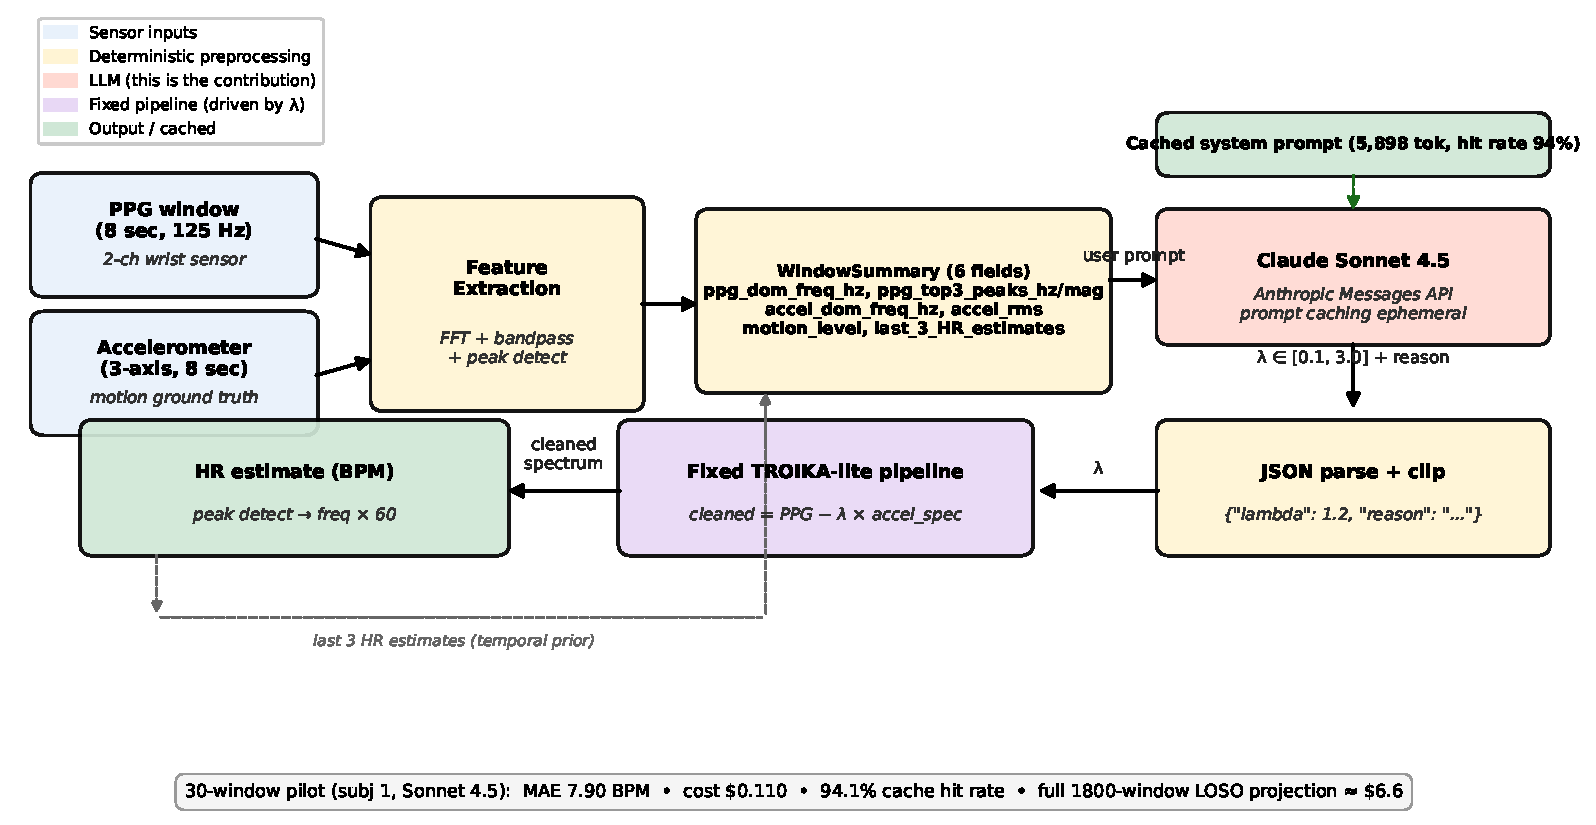
\includegraphics[width=0.94\textwidth]{architecture.pdf}
\caption{System architecture for the $\lambda$-generator (Route~C). Per window, deterministic preprocessing (FFT + bandpass + peak detect) extracts a 6-field numerical summary that is sent as a short user prompt to Claude Sonnet~4.5 alongside a cached system prompt (5{,}898 tokens, hit rate 94\%). Claude returns a single $\lambda \in [0.1, 3.0]$ which then drives a fixed TROIKA-lite spectral-subtraction pipeline. The last 3 HR estimates are fed back into the next window's summary as a temporal prior.}
\label{fig:arch}
\end{figure*}

\begin{figure}[t]
\centering
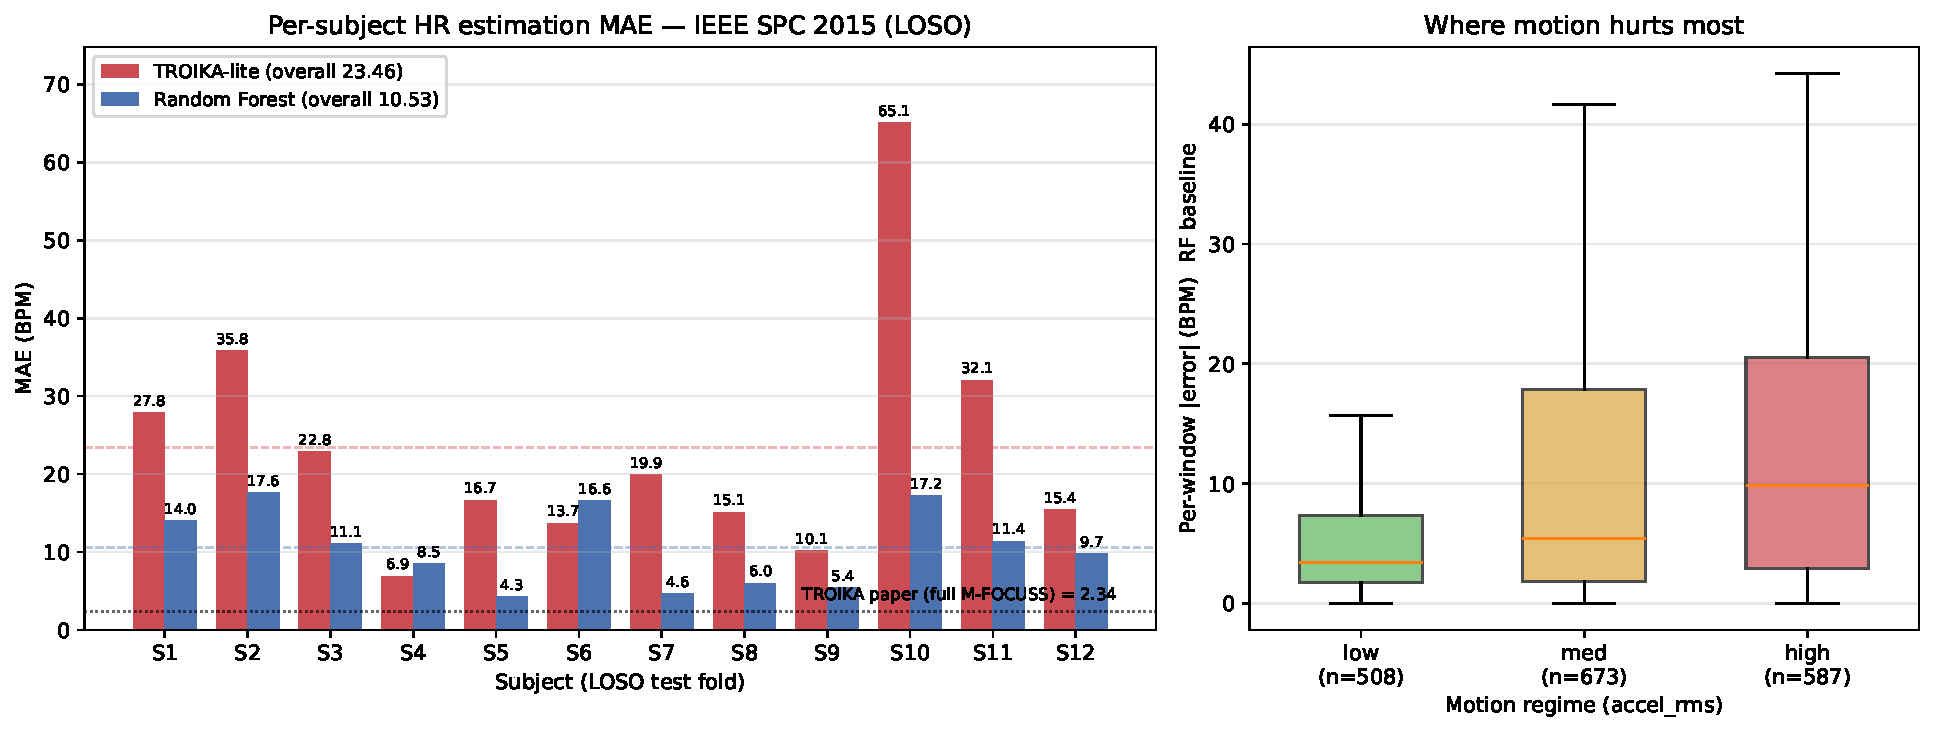
\includegraphics[width=\columnwidth]{baselines_comparison.pdf}
\caption{Baseline comparison on full 12-subject LOSO. \textbf{Left:} per-subject MAE (TROIKA-lite vs.\ Random Forest); the dotted line marks the original TROIKA paper's 2.34 BPM with full M-FOCUSS. \textbf{Right:} RF per-window error stratified by motion regime; high-motion windows (accelerometer RMS $\ge$~1.7) carry the largest errors and are the regime where the LLM $\lambda$-generator is hypothesized to help.}
\label{fig:baselines}
\end{figure}

\begin{figure}[t]
\centering
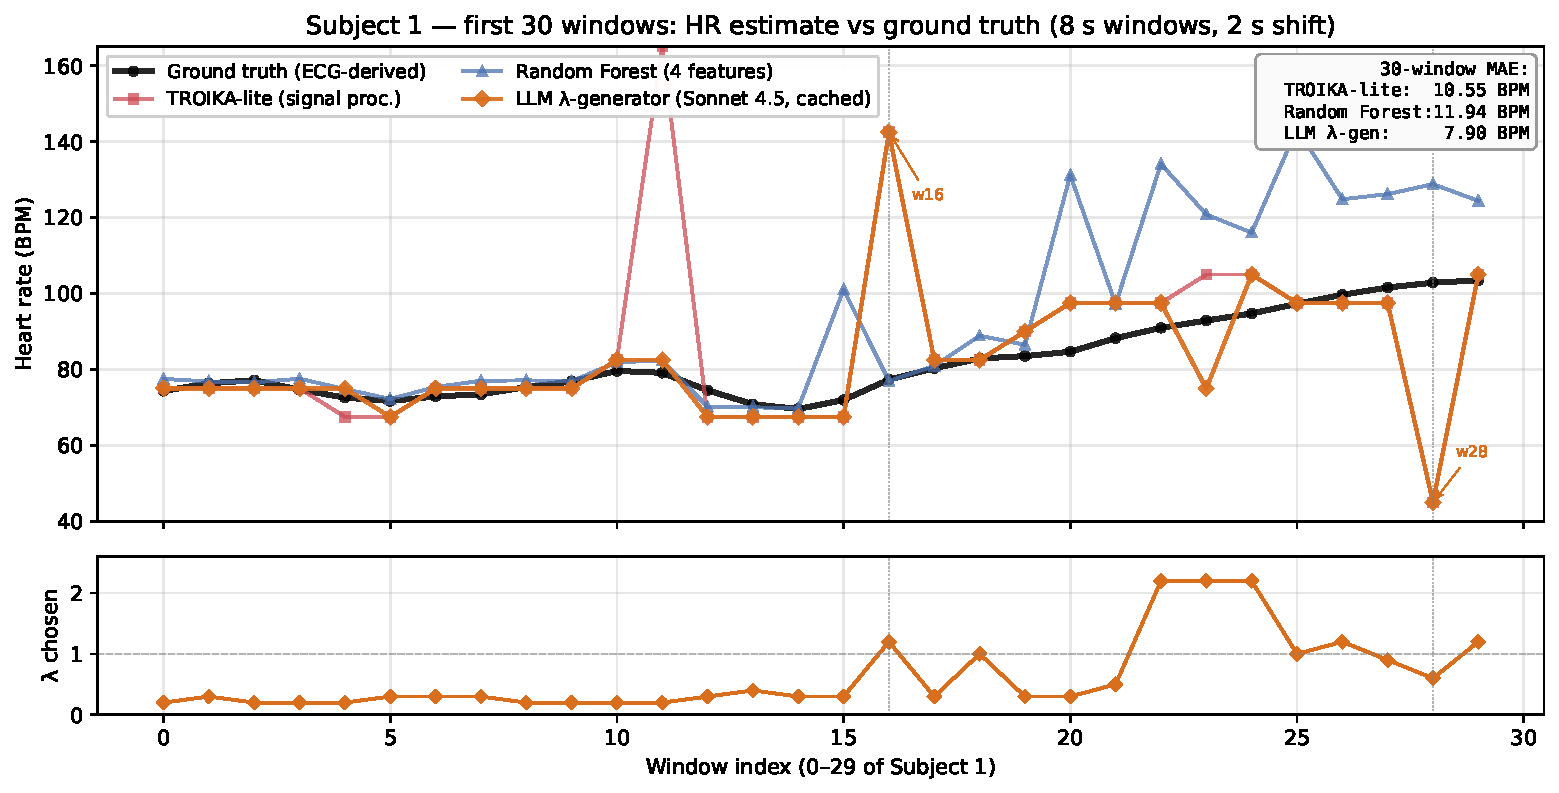
\includegraphics[width=\columnwidth]{pilot_subj1_comparison.pdf}
\caption{30-window pilot on Subject~1, all three systems on the same windows. \textbf{Top:} HR estimates vs.\ ground-truth ECG-derived HR. \textbf{Bottom:} the per-window $\lambda$ chosen by the LLM. The LLM uses small $\lambda$ (0.2--0.4) during low-motion windows 0--14 and increases $\lambda$ (range 0.6--2.2) as motion picks up after window 22; outlier windows w16 and w28 (annotated) account for most of the residual MAE.}
\label{fig:pilot}
\end{figure}

% ─────────────────────────── REFERENCES ───────────────────────────
\bibliographystyle{ACM-Reference-Format}
\bibliography{references}

\end{document}
